
Para el estudio del m\'etodo de generaci\'on de OFC mediante \gs\ se ha trabajado con una corriente de inyecci\'on $I(t)$ modulada mediante una función sinusoidal superpuesta a una corriente de polarización $\ibias$ con la expresi\'on de la ecuación \ref{eq:gainSwtching}.

	Tal y como se vi\'o en el apartado \ref{Intr:OFC:GS} la calidad del \gs\ viene dada tanto por la intensidad de los picos como por la duraci\'on del pulso. De esta manera, se ha procedido a caracterizar los peines \'opticos de frecuencia en funci\'on del \gs\ aplicado modificando la frecuencia de oscilaci\'on y la amplitud de la corriente inyectada. Para el estudio del \gs\ en función de la frecuencia de oscilaci\'on se ha modificado el valor de $f_R$, estudiando primero los OFC para altas frecuencias ($f_R = 5.0$ GHz) y luego para bajas frecuencias ($f_R = 500$ MHz). Cabe destacar que al variar el valor de la frecuencia de oscilaci\'on $f_R$, la impedancia del l\'aser $Z_l$ tambi\'en cambia y as\'i también la suma $Z_0 + Z_l$.

	Para ambos valores de frecuencias $f_R$ se han estudiado los efectos producidos al variar la amplitud de la corriente de inyecci\'on, comparando tanto los espectros ópticos obtenidos como las variables dinámicas para diferentes amplitudes. Para el estudio con diferentes amplitudes ha bastado con modificar los valores de $V_{RF}$, ya que $(Z_0 + Z_l)$ solo varia para la frecuencia.

	\addtocontents{toc}{\vspace{0.1cm}}
	\subsection{Efecto de la amplitud de modulación a altas frecuencias}
		\label{Sol:OFC:HgFreq}

		Para el estudio del efecto de la amplitud de modulación a altas frecuencias se ha trabajado con una corriente de polarización $\ibias = 30$ mA y una frecuencia $f_R = 5.0$ GHz. Tal y como se vi\'o en el apartado \ref{Sol:CW:RoF}, la frecuencia de oscilaciones de relajación del l\'aser para $\ibias = 30$ mA es de $\nu_{RoF} \approx 5.9$ GHz, del orden de $f_R$. Se han resuelto las ecuaciones de balance, obteniendo los OFC para tres amplitudes diferentes con $V_{RF}$: $0.05$ V, $1.00$ V y $1.50$ V. 

		En la Figura \ref{Img:rateEquations} se muestra la evolución temporal de la \I, la \s, la \n\ y de \chirp\ para varios valores de $V_{RF}$ pasada la zona del transitorio.

			% Img:rateEquations
			\begin{figure}[H]
				\centering
				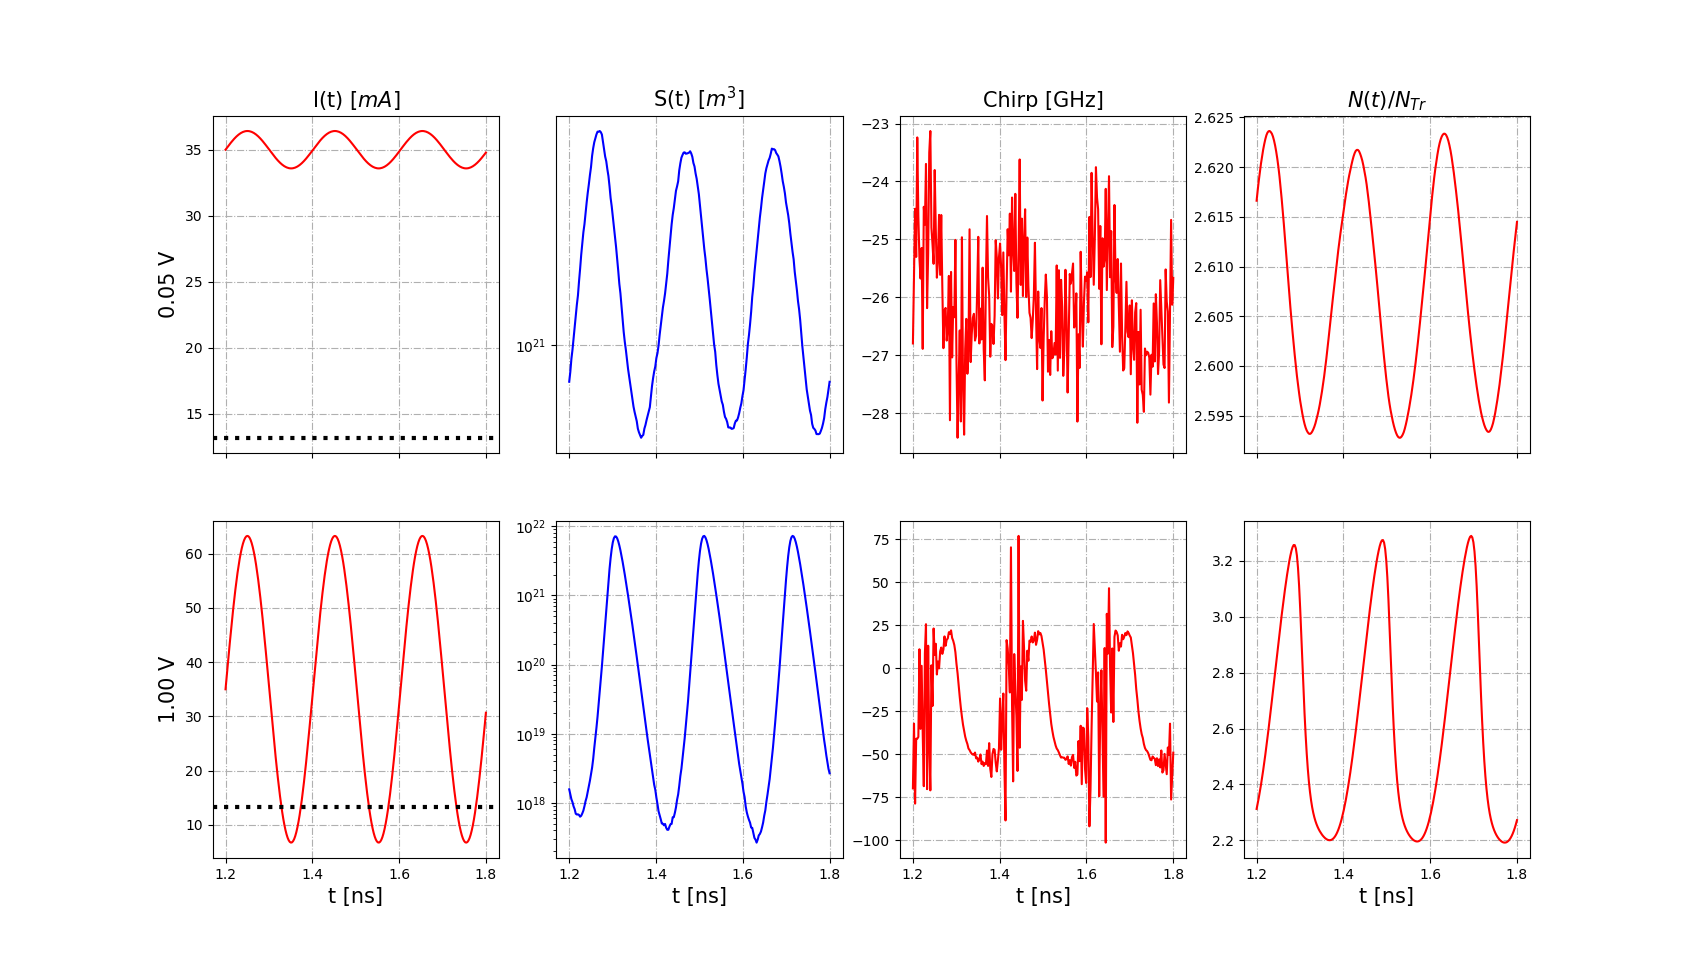
\includegraphics[width=1.0\linewidth]{rateEquations.png}
				\caption{\label{Img:rateEquations}Evolución temporal de \I ((a)-(c)), \s ((d)-(f)), \n\ ((g)-(i)) y \chirp\ ((j)-(l)) en funci\'on de $V_{RF}$ pasada la zona del transitorio. Para la \I\ se ha marcado la corriente umbral del l\'aser $I_{th} = 14.8$ mA con una l\'inea horizontal discontinua. En la primera columna se muestran las evoluciones temporales para una amplitud de la corriente equivalente a $V_{RF} = 0.05$ V (verde), en la segunda columna para $V_{RF} = 1.00$ V (azul) y en la tercera columna de $V_{RF} = 1.50$ V(naraja).}	
			\end{figure}

		Mientras que para el caso del l\'aser en corriente continua ($I(t) = \ibias$) estudiado en la secci\'on anterior (secci\'on \ref{Sol:CW}), $S(t)$, $N(t)$ y el \chirp\ alcanzaban un valor constante pasado el transitorio, ahora la modulación en la corriente produce oscilaciones de igual periodo en $S(t)$, $N(t)$ y el \chirp. Se observa un aumento de la amplitud en $S(t)$, $N(t)$ y el \chirp\ al aumentar la amplitud de la corriente. Adem\'as, se observa como las oscilaciones en $N(t)$ y el \chirp\ van en fase (m\'aximos en el mismo tiempo $t$), mientras que los m\'aximos de $S(t)$ se obtienen cuando $N(t)$ decae a $N_{th}$.
			
		Para el caso de $V_{RF} = 0.05$ V, con una menor amplitud, se observa que las oscilaciones en la corriente (Figura \ref{Img:rateEquations} (a)) son pequeñas. Al igual que la corriente; la \s, la \n\ y el \chirp\ tambi\'en presentan oscilaciones de amplitud pequeña.

		Al aumentar la amplitud de la corriente a $V_{RF} = 1$ V (Figura \ref{Img:rateEquations} (b)) se observa como los aumentos de la corriente durante la oscilaci\'on coinciden con el crecimiento de \n\ (Figura \ref{Img:rateEquations} (k)), haciendo que tome valores muy superiores a $N_{th}$. A su vez, esto produce que, al superar $N(t)$ el valor del umbral $N_{th}$, la \s\ (Figura \ref{Img:rateEquations} (e)) tambi\'en tenga un pico superior al valor del l\'aser en corriente continua. De igual forma que ocurría en el transitorio, al aumentar $S(t)$ y dominar la emisi\'on estimulada, $N(t)$ comienza a disminuir, alcanzando un m\'aximo. Sin embargo, en el momento en el que $N(t)$ alcanza el m\'inimo, la corriente se encuentra por debajo de la corriente umbral $I_{th}$, y $N(t)$ no puede aumentar hasta que $I(t)$ toma nuevamente valores mayores de $I_{th}$. Hay un intervalo de tiempo en que $S(t)$ es pequeño pero a\'un lo suficientemente grande como para estar por encima del nivel de emisi\'on espont\'anea. Por tanto, a\'un la emisi\'on estimulada es lo suficientemente intensa para mantener una evoluci\'on principalmente determinista de las variables y, por tanto, coherencia entre los pulsos. La evoluci\'on no es totalmente determinista, pues como se puede apreciar en \ref{Img:rateEquations} (h) el ruido de emisi\'on espont\'anea comienza a afectar al chirp cuando $S(t)$ es pequeña.
		
		Para la amplitud de $V_{RF} = 1.5$ V se observa la misma tendencia que para $V_{RF} = 1$ V, a excepci\'on de que en este caso, al aumentar la amplitud aumenta el tiempo en el que la corriente es menor que $I_{th}$ y as\'i el tiempo en el que $S(t)$ es pequeño y ruidoso debido a que la emisi\'on espontánea ya domina la evolución.


		En la Figura \ref{Img:PSD} se muestran los espectros de los OFC obtenidos mediante \gs\ para las tres amplitudes de la Figura \ref{Img:rateEquations}.

			% Img:PSD
			\begin{figure}[H]
				\centering
				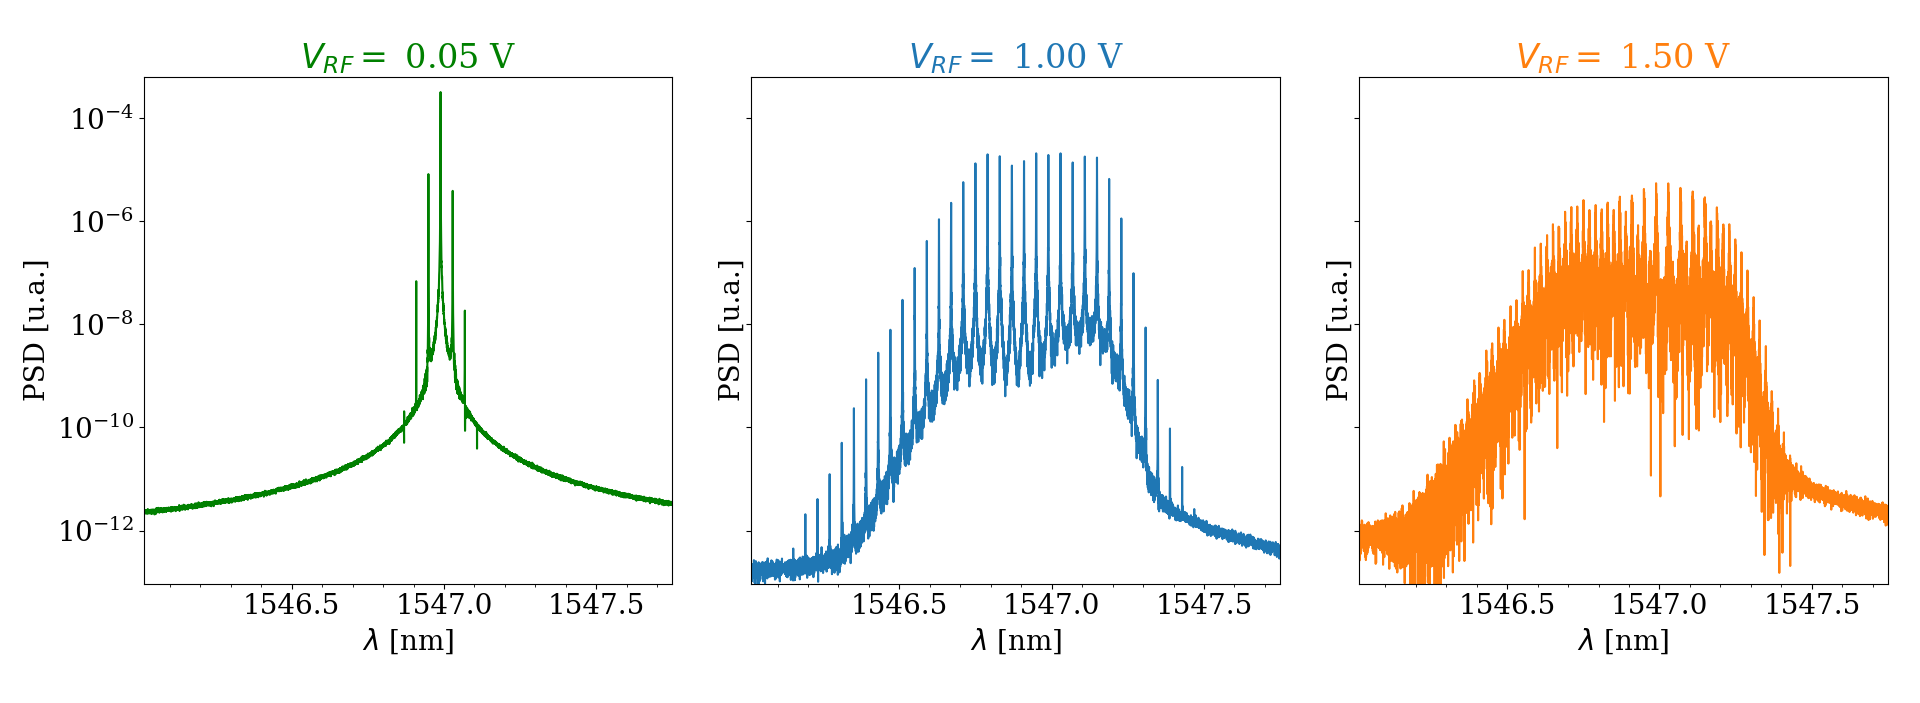
\includegraphics[width=1.0\linewidth]{PSD.png}
				\caption{\label{Img:PSD}Espectros de los OFC obtenidos mediante \gs\ para $\ibias = 30$ mA, $f_R = 5$ GHz y amplitud de modulaci\'on $V_{RF} = 0.05$ V (verde), $1.00$ V (azul) y $1.50$ V (naranja).}
			\end{figure}
			
		Al igual que se obtuvo en la Figura \ref{Img:rateEquations}, se puede observar como el caso de la amplitud de modulaci\'on $V_{RF} = 0.05$ V se asemeja al del l\'aser en corriente cont\'inua, obteniendo un espectro (Figura \ref{Img:PSD} (verde)) con la frecuencia de emisi\'on dominante de la Figura \ref{Img:spectrosCW}. Como consecuencia del \gs\ realizado se observan excitadas líneas de emisión nuevas a los lados de la emisi\'on principal, cuya separación en frecuencias ópticas entre líneas consecutivas es $f_R$ (5 GHz que corresponden a 0.04 nm).

		Para el caso de $V_{RF} = 1$ V se observa un OFC (Figura \ref{Img:PSD} (azul)) de gran calidad formado por numerosas l\'ineas de emisión equiespaciadas (en 5 GHz) y bien definidas. Están bien definidas pues aún se mantiene la coherencia entre pulsos (Figura \ref{Img:rateEquations} (e)) y el ancho del espectro aumenta con respecto al de $V_{RF} = 0.05$ V porque los pulsos ópticos son mucho más estrechos (ver Figuras \ref{Img:rateEquations} (d) y \ref{Img:rateEquations}(e)). Se ha obtenido una regi\'on de longitudes de onda con l\'ineas de emisión con máximos de la densidad espectral de potencia similares, lo cuál es deseable para obtener OFC de buena calidad.

		Por otro lado, se observa que para el caso de $V_{RF} = 1.5$ V (Figura \ref{Img:PSD} (naranja)) el OFC se destruye debido al mayor efecto del ruido de emisión espont\'anea, obteniendo l\'ineas de emisión poco definidas, con un espaciado variado y mucho ruido.

		De esta forma, se ha podido caracterizar la calidad de los OFC, y del \gs, para altas frecuencias en función de la amplitud de modulaci\'on. Se ha podido observar la creaci\'on del OFC para $V_{RF} = 1$ V, as\'i como la destrucci\'on de éste para amplitudes altas, con $V_{RF} = 1.5$ V. Estos resultados coinciden con los observados experimentalmente \cite{artSim}.

		Tal y como se ha comentado a partir de los resultados de la Figura \ref{Img:rateEquations}, uno de los efectos de aumentar la amplitud de modulaci\'on es la disminuci\'on de la corriente por debajo de $I_{th}$ por un tiempo $t$, que aumenta con la amplitud. Sin embargo, \'esto también se puede controlar para una amplitud fija, variando la corriente de polarizaci\'on $\ibias$.

		En la Figura \ref{Img:current} se muestran la potencia $P(t)$, obtenida a partir de la \s\ \ref{eq:Power}, y los espectros de los OFC con $f_R = 5$ GHz, $V_{RF} = 1$ V e $\ibias = 30$ mA y $50$ mA.

			% Img:current
			\begin{figure}[H]
				\centering
				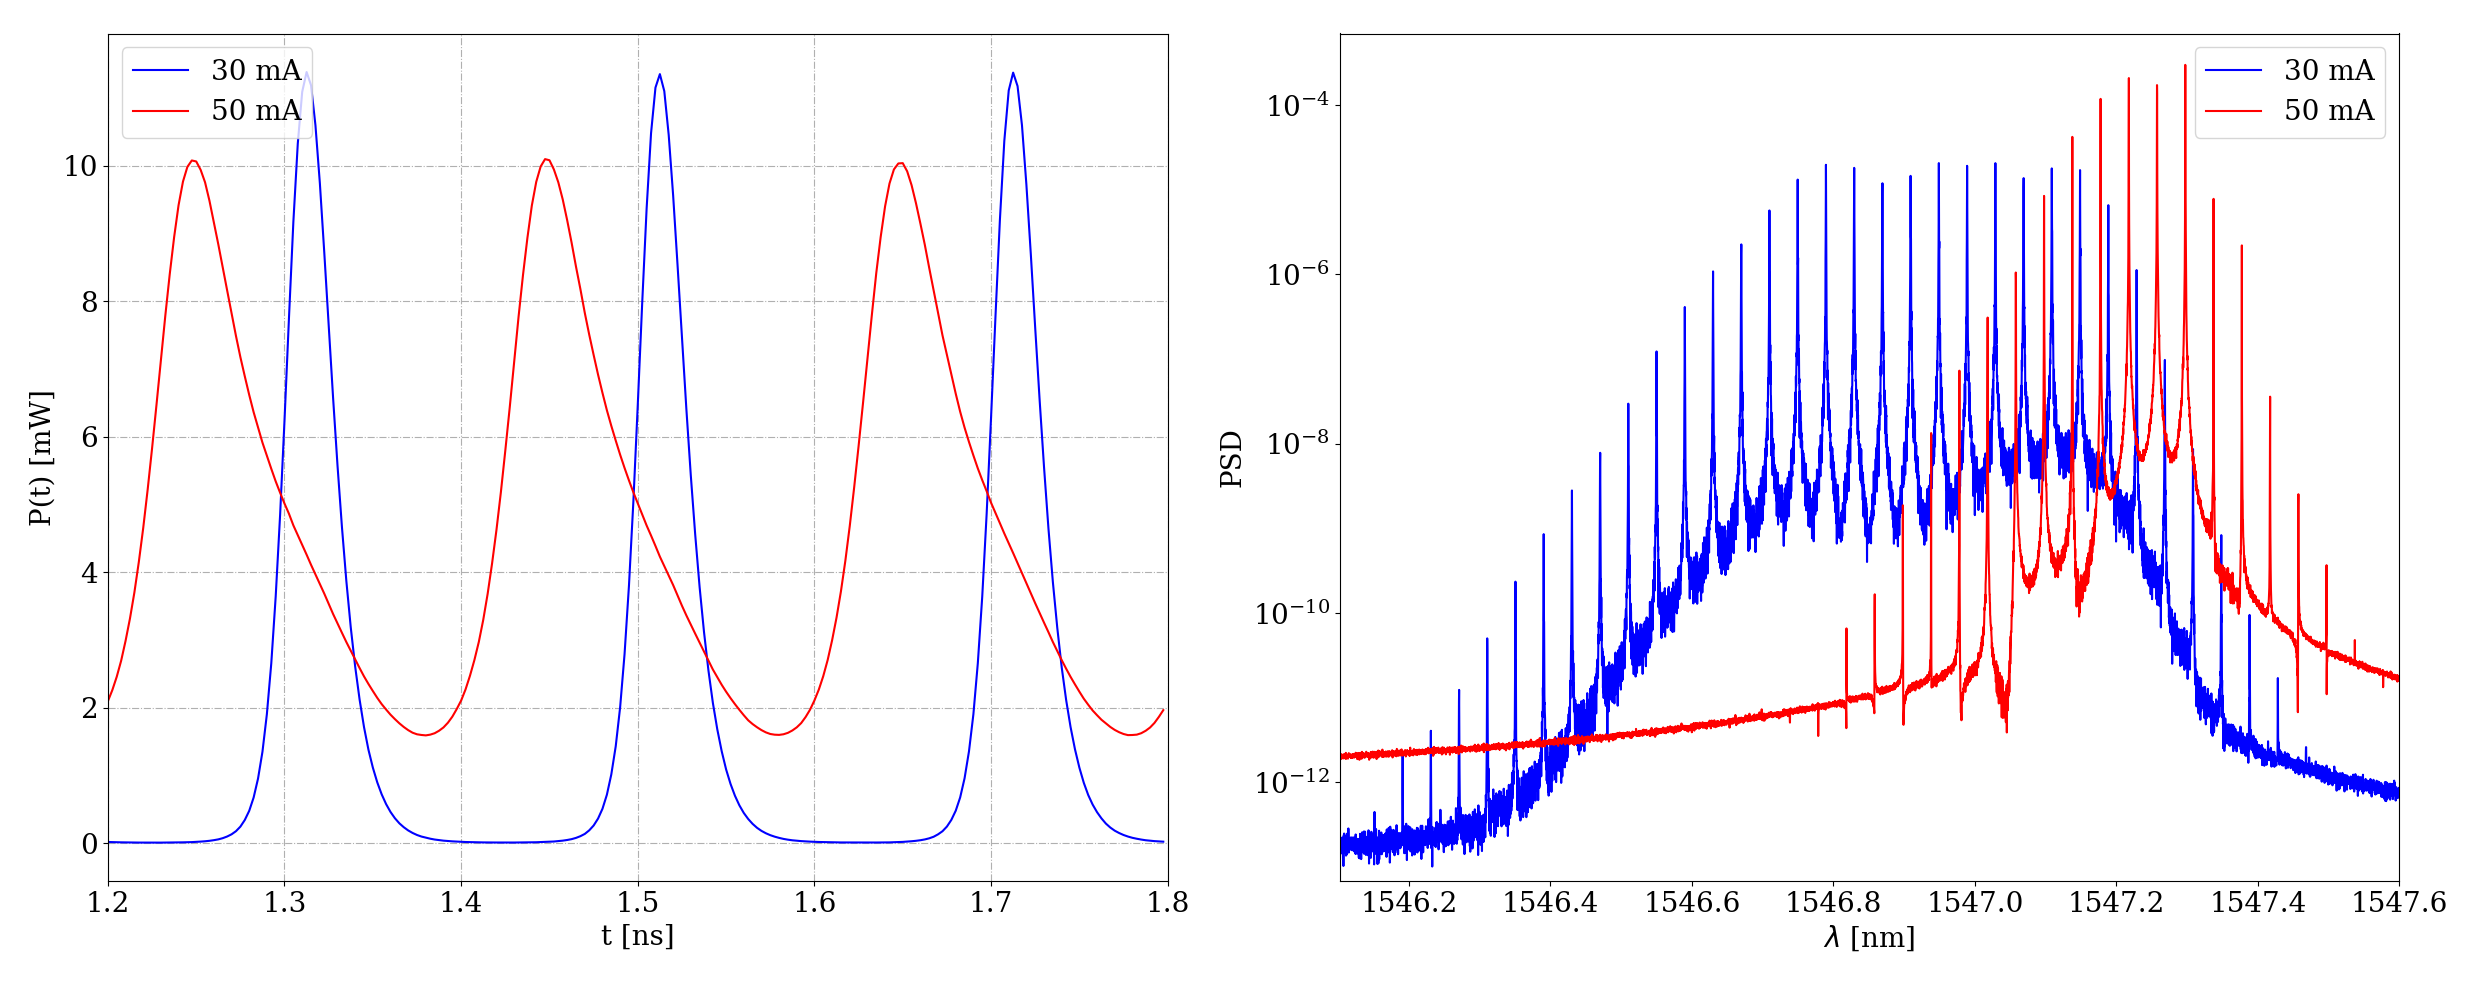
\includegraphics[width=1.0\linewidth]{current.png}
				\caption{\label{Img:current}Perfil temporal de las potencias $P(t)$ (izquierda) y espectros (derecha) de OFC con $f_R = 5$ GHz, $V_{RF} = 1$ V e $\ibias = 30$ mA (azul) y $50$ mA (naranja).}	
			\end{figure}

		El caso de $\ibias = 30$ mA es el ya ilustrado en las Figuras \ref{Img:rateEquations} (e) y \ref{Img:PSD} (azul). En el caso de $\ibias = 50$ mA, al aumentar la corriente de polarizaci\'on, \'esta desplaza la función sinusoidal de la intensidad alejandola de $I_{th}$ y as\'i la amplitud de modulaci\'on no es suficiente para llegar a cruzar $I_{th}$. Esto se observa en el perfil temporal de $P(t)$ (Figura \ref{Img:current} (izquierda, naranja)) que no toma nunca valores cercanos a cero. Puesto que la frecuencia $f_R$ y la amplitud $V_{RF}$ de modulación s\'i son suficientes como para que se d\'e \gs, se observa un espectro (Figura \ref{Img:current} (derecha, naranja)) con un OFC formado por l\'ineas bien definidas e igualmente espaciadas. No obstante, el OFC obtenido para $\ibias = 50$ mA es m\'as estrecho que el obtenido para $\ibias = 30$ mA, pues los pulsos son más anchos para $\ibias = 50$ mA careciendo de una meseta bien definida con l\'ineas de emisi\'on con densidad espectral de potencia similar. Se observa además un corrimiento hacia el rojo del espectro cuando la corriente aumenta cuyo origen es el mismo que el discutido en la Figura \ref{Img:spectrosCW}.

		Otro de los efectos de aumentar la $\ibias$ de tal manera que no cruce la $I_{th}$ es la falta de una regi\'on donde domine la emisi\'on espont\'anea, como ocurría en la Figura \ref{Img:rateEquations}. Esto se puede observar en el menor ruido obtenido en el espectro para $\ibias = 50$ mA (Figura \ref{Img:current} (derecha, naranja)) frente al obtenido en el espectro de $\ibias = 30$ mA (Figura \ref{Img:current} (derecha, azul)).

	\addtocontents{toc}{\vspace{0.1cm}}
	\subsection{Efecto de la amplitud de modulación a bajas frecuencias}
		\label{Sol:OFC:LwFreq}

		Para el estudio del efecto de la amplitud de modulación a bajas frecuencias se ha trabajado con una corriente de polarización $\ibias = 50$ mA y una frecuencia $f_R = 500$ MHz. Se han obtenido en la Figura \ref{Img:500} la potencia $P(t)$ y los espectros ópticos para cuatro amplitudes diferentes, tomando cuatro valores distintos para $V_{RF}$: $0.05$ V, $0.4$ V, $1.0$ V y $1.2$ V.

			% Img:500
			\begin{figure}[H]
				\centering
				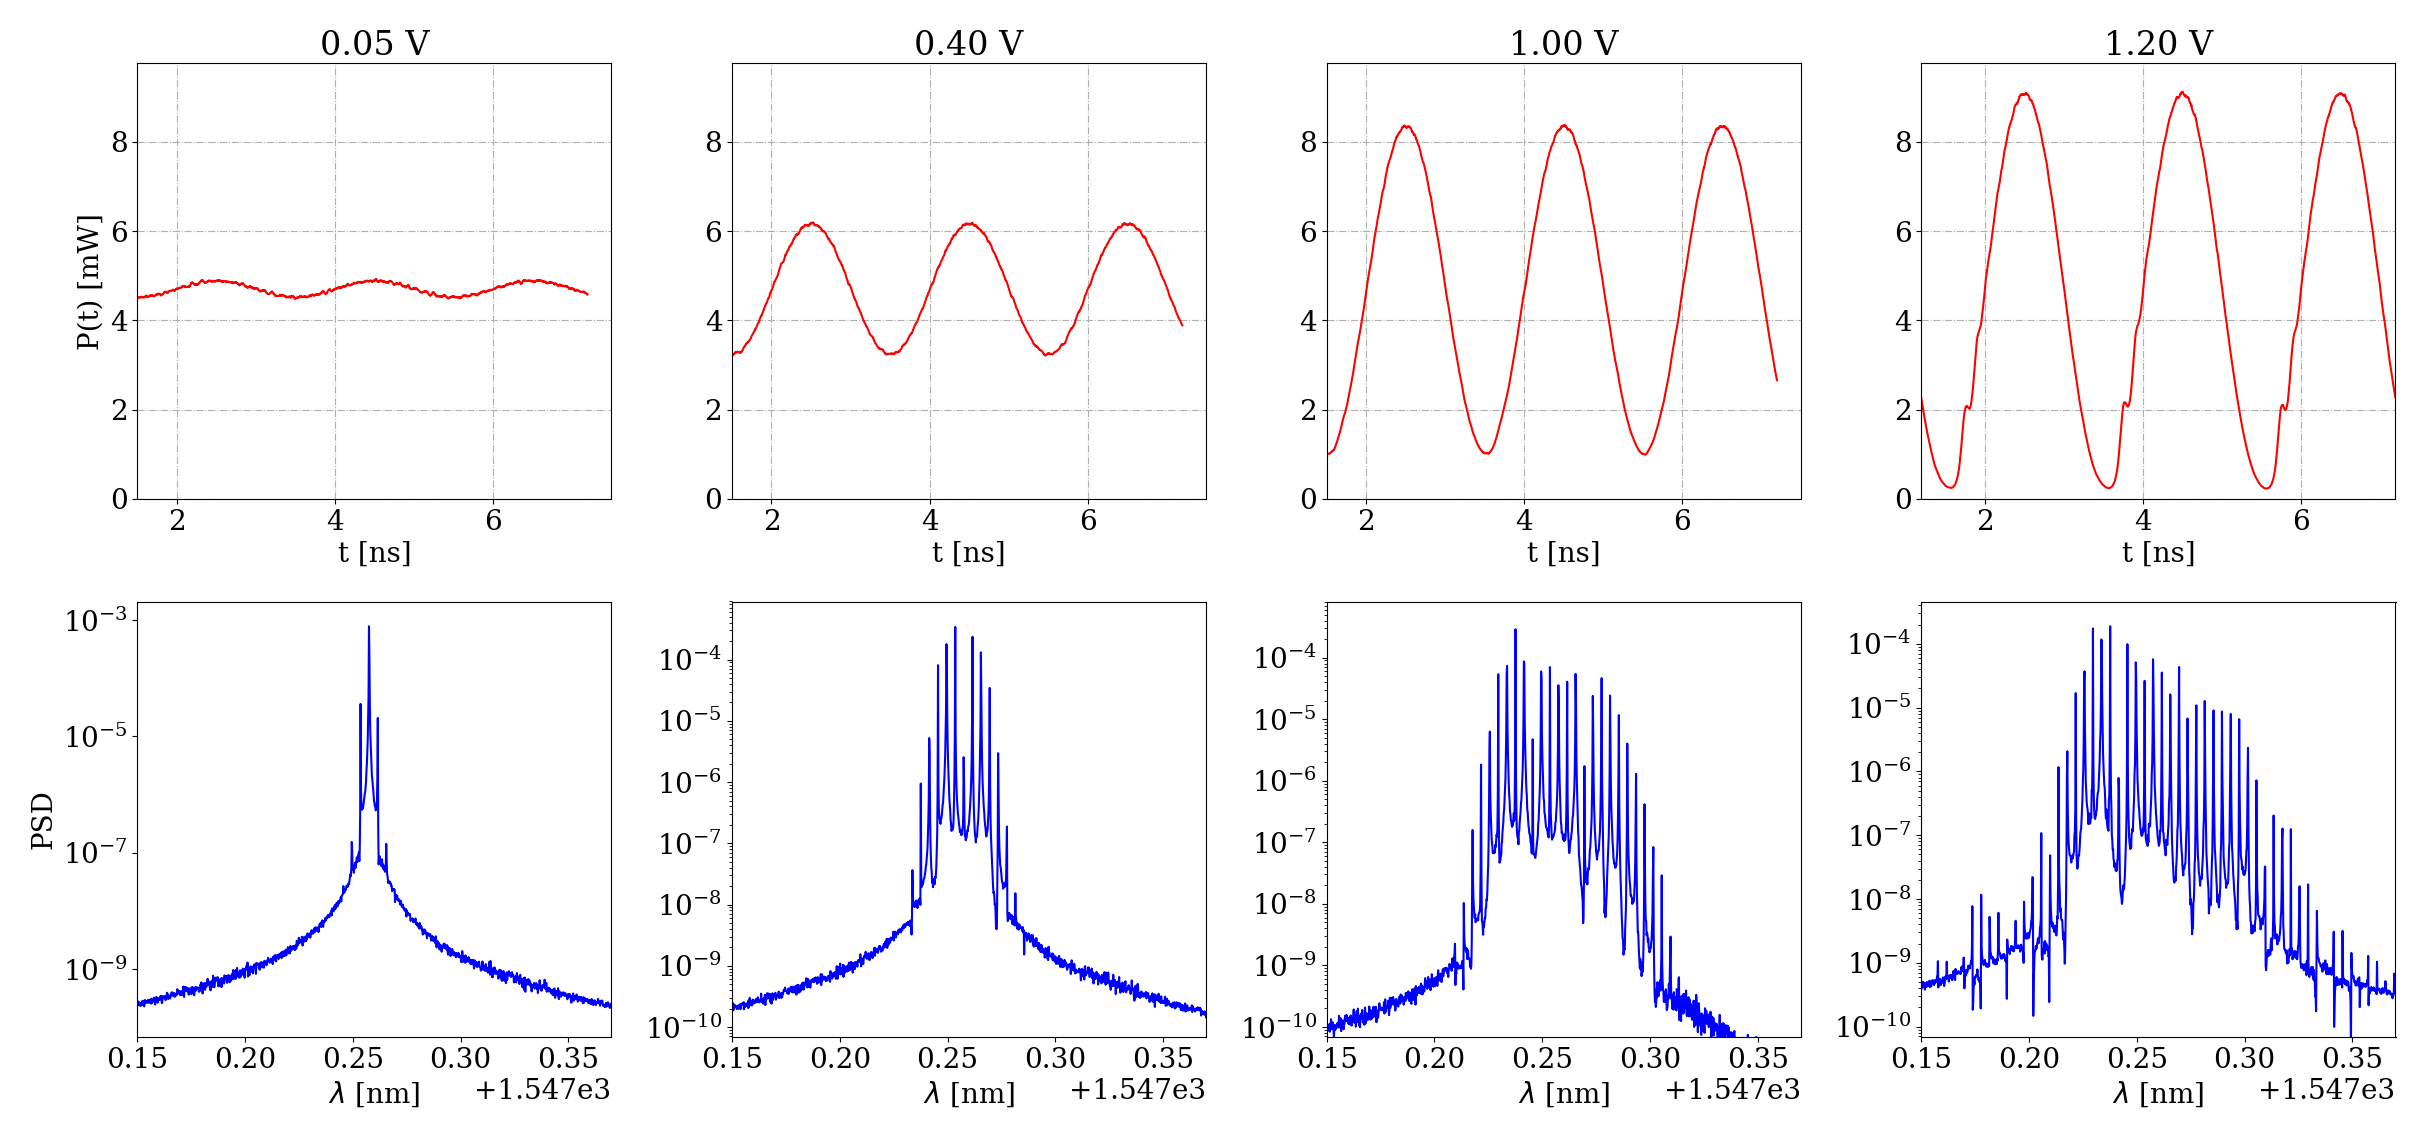
\includegraphics[width=1.0\linewidth]{500.png}
				\vspace{-0.5cm}
				\caption{\label{Img:500}Perfiles temporales de la potencia $P(t)$ (fila superior) y espectros (fila inferior) de los OFC para $\ibias = 50$ mA, $f_R = 500$ MHz y $V_{RF} = 0.05$ V (primera columna), $0.4$ V (segunda columna), $1.0$ V (tercera columna) y $1.2$ V (cuarta columna).}	
			\end{figure}

		Al igual que se obtuvo en el apartado anterior para el caso de altas frecuencias con $\ibias = 50$ mA (Figura \ref{Img:current}), se observan en la Figura \ref{Img:500} perfiles temporales de la potencia oscilantes entorno al valor de la potencia en corriente continua ($P_{CW} \approx 4.7$ mW), variando su amplitud en funci\'on de la amplitud de modulación. Al tener una $\ibias$ muy superior a $I_{th}$ y una frecuencia baja, la amplitud de modulaci\'on no permite mantener la corriente de inyecci\'on por debajo de la corriente umbral un tiempo suficiente como para que $P(t) \propto S(t) \approx 0$, tal y como se observa en las Figuras \ref{Img:500} (fila superior).

		Para el caso de la amplitud de modulaci\'on pequeña con $V_{RF} = 0.05$ V, se ha obtenido un comportamiento muy similar al de corriente continua, al igual que para altas frecuencias. El espectro obtenido para esta amplitud de modulaci\'on es similar al de la Figura \ref{Img:PSD} (verde) del apartado anterior, obteniendo un pico de emisi\'on dominante correspondiente a la emisi\'on en continua y dos picos a cada lado debidos a la modulación sinusoidal de la corriente. La separación entre líneas adyadientes es la que corresponde a una frecuencia óptica igual a $f_R$.

		Se observa como, al igual que ocurría en a altas frecuencias, a medida que aumenta la amplitud de modulación aumenta el n\'umero de l\'ineas de emisión de espectro, llegando a destruirse para altas amplitudes de modulación. Sin embargo, al trabajar a bajas frecuencias se observa una clara irregularidad en el perfil del OFC, tomando los picos valores muy diversos de la densidad espectral de potencia. Tambi\'en cabe destacar la aparici\'on de unos pequeños picos en la base del perfil temporal de la potencia para $V_{RF} = 1.2$ V. Esto se debe al comienzo de la excitación del primer pico de las oscilaciones de relajación.		

		En la Figura \ref{Img:500mhz} se muestran los perfiles temporales de la potencia $P(t)$ y los espectros de los OFC para $\ibias = 50$ mA, $f_R = 500$ MHz y $V_{RF} = 0.1$ V, $0.4$ V, $1.2$ V y $1.6$ V obtenidos experimentalmente \cite{Chaves19}, permitiendo comparar los resultados obtenidos mediante simulación con los obtenidos en el laboratorio.

			% Img:500mhz
			\begin{figure}[H]
				\centering
				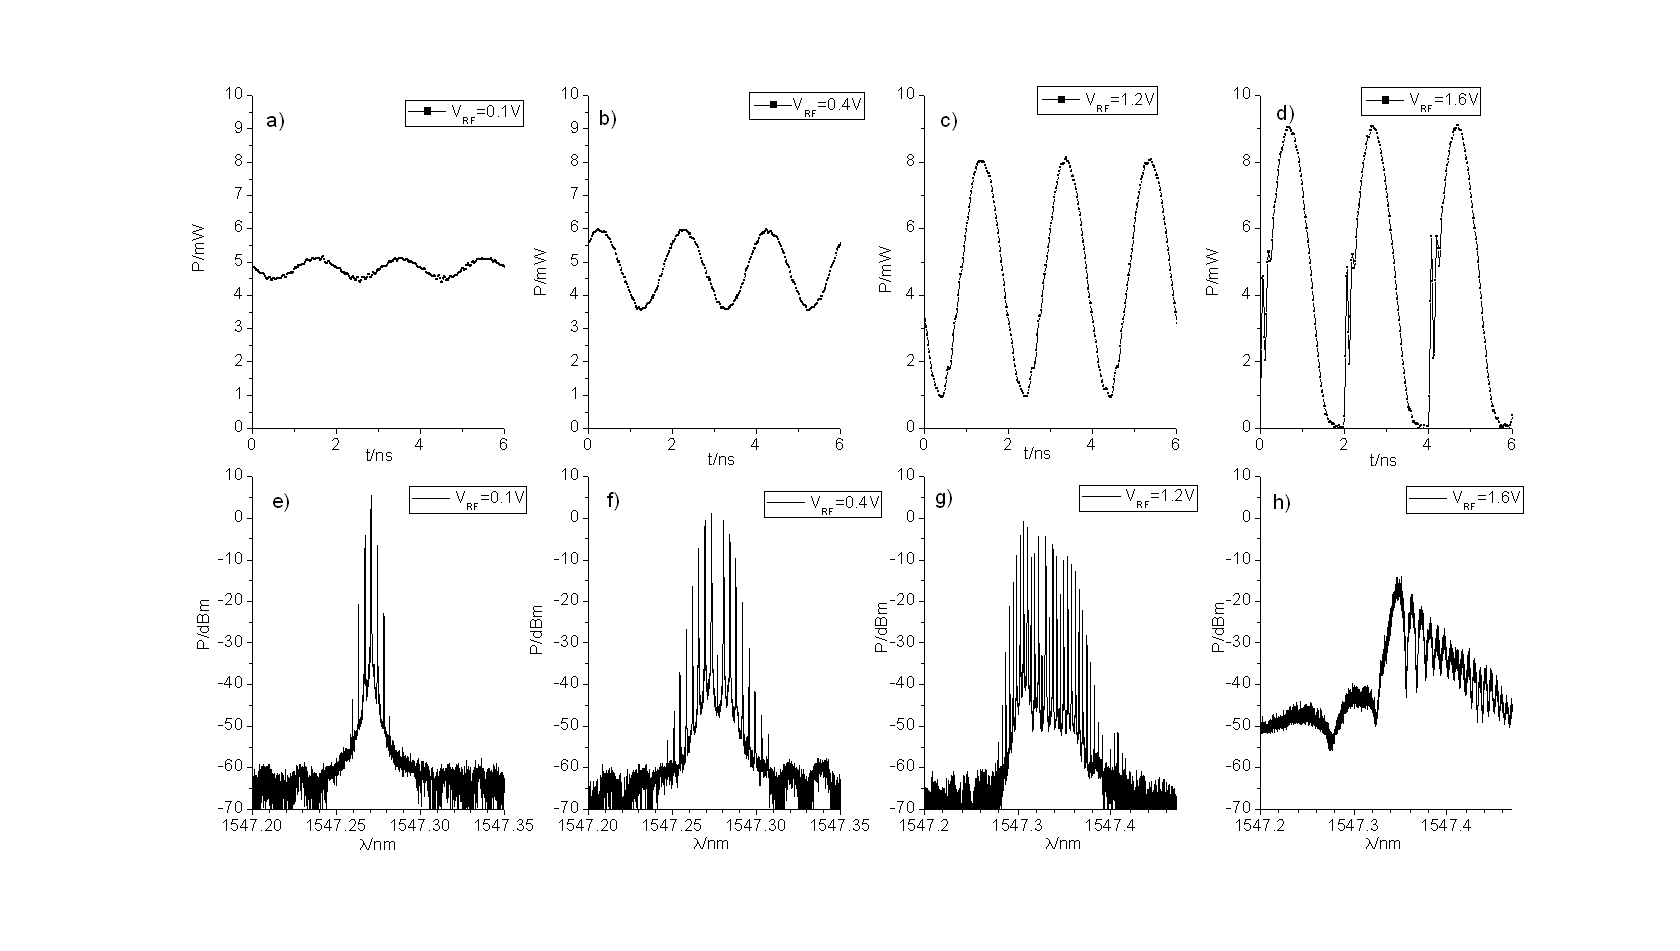
\includegraphics[width=1.0\linewidth]{../Chaves/OFC-GS/500mhz.png}
				\vspace{-1.5cm}
				\caption{\label{Img:500mhz}Perfiles temporales de la potencia $P(t)$ (fila superior) y espectros (fila inferior) de los OFC para $\ibias = 50$ mA, $f_R = 500$ MHz y $V_{RF} = 0.1$ V (primera columna), $0.4$ V (segunda columna), $1.2$ V (tercera columna) y $1.6$ V (cuarta columna) obtenidos experimentalmente \cite{Chaves19}.}	
			\end{figure}

		En la cuarta columna de la Figura \ref{Img:500mhz} se muestran los resultados obtenidos para una amplitud de $V_{RF} = 1.6$ V, observando como el OFC se encuentra completamente destruido debido a que los pulsos se apagan completamente en contraste con lo observado para $V_{RF}$ más pequeñas. Con dicha amplitud se obtienen en las trazas temporales de la potencia los primeros picos de las oscilaciones de relajaci\'on. En la primera columna de la Figura \ref{Img:500mhz} se muestran los resultados para una amplitud de modulación pequeña de $V_{RF} = 0.1$ V. Al igual que en los resultados de la simulación, se obtiene un comportamiento similar al de la corriente continua con un pico de emisi\'on dominante. No obstante, al tratarse del doble de la amplitud utilizada en la simulaci\'on de la Figura \ref{Img:500} se obtienen un mayor n\'umero de picos de emisión estimulados. Los resultados que se muestran en la segunda columna de la Figura \ref{Img:500mhz}  para $V_{RF} = 0.4$ V equivalen a los resultados de la simulación de la segunda columna de la Figura \ref{Img:500}. En ambas figuras se pueden observar un OFC con un perfil aproximadamente sim\'etrico con un pico de menor intensidad en el centro. Por \'ultimo, la tercera columna de la Figura \ref{Img:500mhz} equivale a la cuarta columna de la Figura \ref{Img:500}, con $V_{RF} = 1.2$ V. Ambos espectros presentan un perfil similar con un aumento brusco de la densidad espectral de potencia de los picos para bajas longitudes de onda, seguido de una disminuci\'on m\'as tenue para lontitudes de onda mayores. En la traza de $P(t)$ de la Figura \ref{Img:500mhz} para dicha amplitud se observan restos de los primeros picos de las oscilaciones de relajaci\'on que se observaban para mayores amplitudes. Dicho resto de los picos tambi\'en se obtenian en la simulaci\'on de la Figura \ref{Img:500}.

	El excelente acuerdo entre los resultados de la simulaci\'on de la Figura \ref{Img:500} y los resultados experimentales de la Figura \ref{Img:500mhz} indican la capacidad de la simulaci\'on de explicar los procesos que involucra el \gs\ en la generaci\'on de OFC, pudiendo servir para la caracterizaci\'on de la calidad de los OFC.
